\documentclass[11pt, oneside]{article} 
\usepackage{geometry}
\geometry{letterpaper} 
\usepackage{graphicx}
	
\usepackage{amssymb}
\usepackage{amsmath}
\usepackage{parskip}
\usepackage{color}
\usepackage{hyperref}

\graphicspath{{/Users/telliott_admin/Dropbox/Tex/png/}}
% \begin{center} 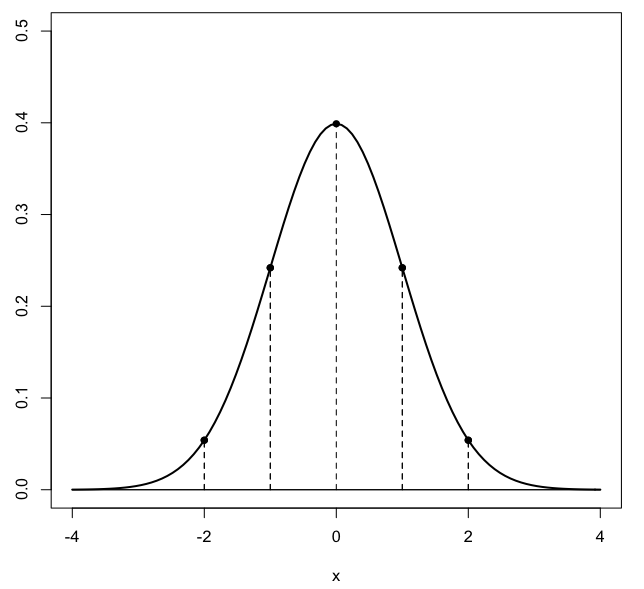
\includegraphics [scale=0.4] {gauss3.png} \end{center}

\title{Moment of inertia}
\date{}

\begin{document}
\maketitle
\Large

Consider a rigid object that rotates about some axis.  Suppose it is nailed down at the axis.  The motion of a point on the object in the plane perpendicular to the axis of rotation will be a circle.

If the radius $r$ to the point from the axis turns through an angle $\theta$, the arc length moved along the perimeter is
\[ s = r \theta \]

We introduce the \emph{angular velocity} $\omega$ as the proportion between the clock time $t$ and the angle $\theta$ turned since time-zero, in units of radians per second:
\[ \theta = \omega t \]
Differentiate both sides with respect to time and the angular velocity can then be seen as the rate of change of the angle
\[ \omega = \frac{d \theta}{dt} \]
Alternatively, use this as the definition of $\omega$ and integrate to obtain $\omega \Delta t = \Delta \theta$.
In Newton's notation we say that $\dot{\theta} = d \theta/dt$ so
\[ \omega = \dot{\theta} \]

In the \hyperref[sec:Uniform_circular_motion]{\textbf{chapter}} on uniform circular motion, we defined the vector $\mathbf{r}$ which goes from the origin to the rotating point.  $\mathbf{r}$ is a function of time, namely:
\[ \mathbf{r} = r \ \langle \cos \omega t, \sin \omega t \rangle \]

The velocity $\mathbf{v}$ is the time-derivative of $\mathbf{r}$:
\[ \mathbf{v} = r \omega \ \langle -\sin \omega t, \cos \omega t \rangle \]

We see that $\mathbf{v} \cdot \mathbf{r} = 0$.  The tangential velocity is perpendicular to the vector $\mathbf{r}$ and it points in the direction of the tangent to the circle at the point.  Its magnitude is
\[ v = r \omega \]
To emphasize its tangential nature we could write $v_T$.

The acceleration is
\[ \mathbf{a} = \frac{d \mathbf{v}}{dt} = -r\omega^2 \ \langle \cos \omega t, \sin \omega t \rangle \]

We say the acceleration due to circular motion is radial, because it points in the (negative) of the same direction as the radius.  Its magnitude is
\[ a = r \omega^2 = r v \]
And again, to emphasize its radial nature we could write $a_r$ but we skip this.

We can also view $v$ at the point as the time-derivative of $s$
\[ v = \frac{d}{dt} s = \frac{d}{dt} r \theta = r \frac{d \theta}{dt} = r \dot{\theta} \]
There is only one term from the product rule since $\dot{r} = 0$, the radius doesn't change with time.  This matches our previous definitions
\[ v = r \omega \]
\[ \omega = \dot{\theta} \]

Going back to the tangential velocity we had
\[ v = r \dot{\theta} = r \omega \]
and the distance moved is
\[ s = r \theta = r \omega t \]

As we said above, for an object turning in a circle at a constant tangential velocity $v$, there is an acceleration toward to the center of the circle.  That acceleration is
\[ a = r \omega^2  \]
\[ = \frac{r^2 \omega^2}{r} = \frac{v^2}{r} \]

If, in addition, the tangential velocity is changing, the tangential acceleration is
\[ a_T = \frac{dv_T}{dt} = \frac{d}{dt} r \omega = r \frac{d \omega}{dt}  \]
Define the angular acceleration $\alpha$ as
\[ \alpha = \frac{d\omega}{dt} =  \ddot{\theta}  \]
Then 
\[ a_T = r \alpha \]

To summarize then:
\[ s = r \theta \]
\[ v_T = r \omega = r \dot{\theta} \]
\[ a_T = r \alpha = r \ddot{\theta} \]

In rotation problems it is useful to think of the angular velocity $\omega$ as an analog of the linear velocity for linear problems.  If we do that, then I, the moment of inertia, plays a role analogous to mass.

Kinetic energy:
\[ K = \frac{1}{2} mv^2 \]
Since $v = r \omega$:
\[ K =  \frac{1}{2} m r^2 \omega^2 \]
Define $I = mr^2$, then
\[ K = \frac{1}{2} I \omega^2 \]

Angular momentum is usually given as the vector product $\mathbf{L} = \mathbf{r} \times \mathbf{p}$, where $\mathbf{p} = m \mathbf{v}$ is the momentum.

If the vectors are at right angles and we just look at the magnitude of the result we have that
\[ L = rp \]
so
\[ L = r mv = r m \ r \omega = I \omega \]

In the same way that the force is the time-derivative of the momentum, the torque $\tau$ is the time derivative of the angular momentum
\[ \tau = \frac{d}{dt} L = I \frac{d \omega}{dt} = I \alpha \]
This is the angular version of Newton's second law $F = ma$.

So with this definition
\[ I = mr^2 \]
we obtain these parallel definitions for angular motion
\[ K = \frac{1}{2} I \omega^2 \]
\[ L = I \omega \]
\[ \tau = I \alpha \]

In a sense, the contribution of the radius is shifted from the velocity component (angular velocity) to the mass component (moment of inertia).

The moment of inertia of a collection of discrete masses is the sum of each mass, times the square of the distance to the chosen axis of rotation.  

\subsection*{rods}
Imagine that we have a uniform (thin) rod, and it's going to rotate around the center of the rod.  Choose the center as the origin of coordinates.  The ends of the rod are then at $-l/2$ and $+l/2$.

Calculate the mass per unit length $M/l$, and so in a tiny sliver of the rod of width $dx$, the mass at that position is $M/l \ dx$ and its moment is $Mx^2/l \ dx$.  We add them all up:
\[ I = \int_{-l/2}^{l/2} \frac{M}{l} x^2 \ dx \]
\[ =  \frac{M}{l} \ \frac{x^3}{3} \bigg |_{-l/2}^{l/2} \]
\[ = Ml^2 (\frac{1}{24} - - \frac{1}{24}) = \frac{1}{12} Ml^2 \]

If we move the axis to the end of the rod, then adjust the coordinate system as well, and we have
\[ \int_0^l \frac{M}{l} x^2 \ dx \]
\[ =  \frac{M}{l} \ \frac{x^3}{3} \bigg |_{0}^{l} = \frac{1}{3} Ml^2 \]  

There is a principle called the \emph{parallel axis} theorem which says that 
\[ I = I_{CM} + md^2 \]
The moment around a different axis is equal to the moment around the $CM$, the center of mass, plus $md^2$ where $d$ is the distance between the two axes.  

The first example was at the $CM$ of the rod, and the distance we moved was $l/2$ so we have
\[ I = \frac{1}{12} Ml^2 + M (\frac{l}{2})^2 = Ml^2 (\frac{1}{12} + \frac{1}{4}) = \frac{1}{3} Ml^2 \]

\subsection*{rings and disks}
Imagine the object is a ring, and we're rotating around the center.  Think of it as a sum of discrete pieces
\[ I = \sum_i m_i r^2 \]
But $r = R$ for every piece so we have
\[ I = R^2 \sum_i m_i = MR^2 \]

For a thin disk, we imagine adding up the contribution for a series of rings with increasing radius.  At radius $r$, the circumference of the ring is $2 \pi r$, and the area of the ring is $2 \pi r \ dr$.  The mass per unit area is $M/\pi R^2$ so the mass of each ring is
\[ m = \frac{M}{\pi R^2} \ 2 \pi r \ dr = \frac{2M}{R^2} r \ dr \]
Integrate mass times radius squared from $r=0 \rightarrow R$
\[ I = \int_0^R r^2 \frac{2M}{R^2} r \ dr \]
\[ = \frac{2M}{R^2} \ \frac{r^4}{4} \bigg |_{0}^{R} =  \frac{1}{2} MR^2 \]
Now, if we were to move the axis of rotation to the edge, we would have
\[ I = \frac{MR^2}{2} + MR^2 = \frac{3}{2} MR^2 \]
\subsection*{sphere}
Start with the sphere.  It's analogous to the ring, but harder.  I struggled with this one, by not using the appropriate slant height when calculating the area of a slice.  I found another approach online:

\url{http://www.miniphysics.com/uy1-calculation-of-moment-of-inertia-of_04.html}

 \begin{center} 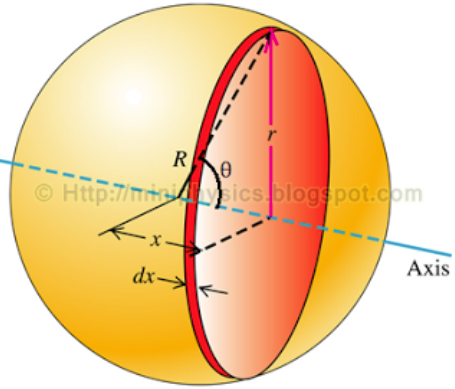
\includegraphics [scale=0.4] {moment_sphere.png} \end{center}

and I liked it so much I want to show that approach.  We slice the sphere perpendicular to the axis of rotation.  For each slice we have a ring of radius $r$ whose moment is
\[ dI = r^2 \ dm \]
where
\[ dm = \frac{M}{A} \ dA = \frac{M}{4\pi R^2} \ dA \]
The trick is to express the area of the ring (parametrize our slices) in terms of an angle $\theta$, shown in the figure ($\theta = 0 \rightarrow \pi$, where $\theta = \pi/2$ is perpendicular to the axis).  Doing this, we get the correct area for the width of the ring, namely $R \ d \theta$, and a total area for the ring of
\[ dA = 2 \pi r \ R \ d \theta \]
so
\[ dm =  \frac{M}{4\pi R^2} \ dA =   \frac{M}{4\pi R^2} \ 2 \pi r \ R \ d \theta =   \frac{M}{2 R} \ r \ d \theta \]
and then
\[ dI = r^2 \ dm =  \frac{M}{2 R} \ r^3 \ d \theta \]
Now, we need to get a relationship between $r$ and $\theta$, but from the diagram it's clear that
\[ r = R \sin \theta \]
so we have the integral
\[ I = \int dI = \frac{MR^2}{2}  \int_0^{\pi} \sin^3 \theta \ d \theta \]
This is pretty easy.  We do
\[ \sin^3 \theta \ d \theta = (1- \cos^2 \theta) \sin \theta \ d \theta \]
the integral is just
\[  \int \sin^3 \theta \ d \theta = - \cos \theta + \frac{\cos^3 \theta}{3} \ \bigg |_0^{\pi} = (1 - \frac{1}{3}) - (-1 + \frac{1}{3}) = \frac{4}{3} \]
and the answer is 
\[ \frac{2}{3} MR^2 \]

\subsection*{solid ball}
With the previous result in hand the solid ball is pretty easy.  We imagine a series of concentric spheres with increasing radius $r = 0 \rightarrow R$.  Each sphere has
\[ dI = \frac{2}{3} dm \ r^2 \]
\[ dm = \frac{M}{4/3 \pi R^3} \ 4 \pi r^2 = \frac{3M}{R^3} r^2 \]
so 
\[ dI = \frac{2M}{R^3} r^4 \]
\[ I = \int \ dI = \frac{2M}{R^3}  \int_0^R r^4 \]
\[ = \frac{2M}{R^3} \ \frac{R^5}{5} = \frac{2}{5} MR^2 \]

\subsection*{parallel axis theorem}
Our first proof of the parallel axis theorem is from Fitzpatrick.  Choose the origin of coordinates to be at the center of mass of the body.  

Orient the $z$-axis with the axis of rotation.  Orient the new axis so that the new moment of inertia lies along the $x$-axis at $x=d; y =0$.

Since the center of mass is at the origin, by definition
\[ \iiint x \ dx \ dy \ dz = 0 \]
with the integral taken over the volume of the body.  The same is true for $y$ and $z$.

The square of the distance of any point in the body from the $z$-axis is $x^2 + y^2$, so the moment of inertia with respect to the center of mass is
\[ I_{CM} = M \frac{\iiint (x^2 + y^2) \ dx \ dy \ dz}{\iiint \ dx \ dy \ dz} \]

The new moment of inertia simply has an additional displacement $d$ with respect to $x$
\[ I' = M \frac{\iiint ((x-d)^2 + y^2) \ dx \ dy \ dz}{\iiint \ dx \ dy \ dz} \]
Expanding and taking the constant $d$ outside the integral
\[ = M \frac{\iiint (x^2 + y^2) \ dx \ dy \ dz}{\iiint \ dx \ dy \ dz} - 2dM \frac{\iiint x \ dx \ dy \ dz}{\iiint \ dx \ dy \ dz} + d^2M \frac{\iiint \ dx \ dy \ dz}{\iiint \ dx \ dy \ dz}\]

We see immediately that the middle integral is zero and the first term is $I_{CM}$ so we have
\[ I' = I_{CM} + d^2M \frac{\iiint \ dx \ dy \ dz}{\iiint \ dx \ dy \ dz}\]
The third term is just $Md^2$
\[ I' = I_{CM} + Md^2 \]
I think this derivation assumes constant density, but it will still work with variable density, just add a function $\delta(x,y,z)$ which never has to be evaluated.

Just in case this fails for some reason that I can't see, let me show you Professor Shankar's version.

We will do this by summation, just pretend we are summing over lots of individual little mass elements with position vectors $\mathbf{r}_i$ from the center of mass.
\[ I_{CM} = \sum_i m_i |\mathbf{r}_i|^2 = \sum_i m_i (\mathbf{r}_i \cdot \mathbf{r}_i) \]
Now we move the axis of rotation to a new position with position vector $\mathbf{d}$ from the center of mass.  Notice that $\mathbf{d}$ will be the same for every $m_i$.  The new moment is
\[ I_{CM}' = \sum_i m_i (\mathbf{r}_i' \cdot \mathbf{r}_i') \] 
where
\[ \mathbf{d} +  \mathbf{r}_i'  = \mathbf{r}_i  \]
\[ \mathbf{r}_i' = \mathbf{r}_i - \mathbf{d} \]
and so
\[ \mathbf{r}_i' \cdot \mathbf{r}_i'  =  (\mathbf{r}_i - \mathbf{d}) \cdot (\mathbf{r}_i - \mathbf{d}) \]
\[ = \mathbf{r}_i \cdot \mathbf{r}_i - 2 \mathbf{r}_i \cdot  \mathbf{d} + \mathbf{d} \cdot \mathbf{d} \]
substitute into the moment calculation
\[ I_{CM}' = \sum_i m_i (\mathbf{r}_i \cdot \mathbf{r}_i) + \sum_i m_i |(-2) \mathbf{r}_i \cdot \mathbf{d} | + \sum_i m_i (\mathbf{d} \cdot \mathbf{d}) \] 
Now, the first term is $I_{CM}$, and in the third term, since $\mathbf{d}$ does not vary with $i$, it is just $d^2$ and we can pull it out of the sum
\[ I_{CM}' = I_{CM} + \sum_i m_i (-2)( \mathbf{r}_i \cdot \mathbf{d}) + d^2 \sum_i m_i \] 
\[ I_{CM}' = I_{CM} + \sum_i m_i (-2)( \mathbf{r}_i \cdot \mathbf{d}) + Md^2 \] 
We're almost there.  We need the middle term to vanish.The coordinates were set up so that $\mathbf{d}$ lies along the $x$-axis, so $ \mathbf{r}_i \cdot \mathbf{d}$ is just the constant $d$ times the $x$-component of $\mathbf{r}_i$ for each vector.
\[ \sum_i m_i (-2)( \mathbf{r}_i \cdot \mathbf{d})  = -2d \sum_i m_i  \mathbf{r}_{ix} \]
$\sum_i m_i  \mathbf{r}_{ix}$ is the $x$-component of the center of mass \emph{in this coordinate system}.  But we've chosen that point to be the origin.  So this term vanishes, leaving
\[ I_{CM}' = I_{CM} + Md^2 \] 

This argument seems to be the same as the first, couched in the language of vectors and using finite sums instead of integrals.

\end{document}  